\chapter{VisualSfM}\label{sec:visualsfm}
%======================================================================================
%
\section*{Introdução}

VisualSfM é um {\it software} baseado em fotogrametria que faz todo o processo de reconstrução 3D de um objeto e que pode usá-lo por linha de comando ou então pela interface gráfica, que é ótima, por sinal. É altamente customizável, podendo utilizar o CUDA da NVIDIA ou OpenGL, especificar a lista de pares para correspondência de imagens, usar detectores de {\it features} próprios, velocidade da detecção de {\it features}, da reconstrução densa, dentre outros parâmetros. Ou seja, é um {\it software} robusto, que pode ser usado em Linux, Windows ou até mesmo Mac.

\section*{Procedimento}

Sua linha de reconstrução é parecida com o MVE \ref{sec:mve}, porém é mais intuitiva. Em sua interface, possui um Log de mensagens e erros que por ventura venham a acontecer e na parte de cima, alguns botões \ref{fig:pipelineVisualSfM}

\begin{figure}[!h]
	\centering

	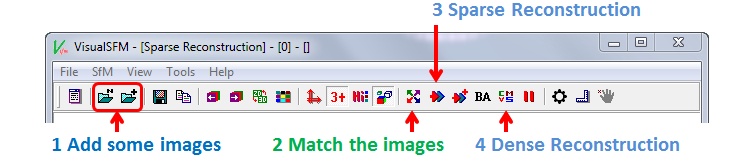
\includegraphics[width=1\linewidth]{figs/pipelinevisualsfm.png}
	\caption{%
	Botões na parte superior da interface gráfica, este seria o {\it pipeline} padrão de funcionamento do {\it software}.
	}\label{fig:pipelineVisualSfM}
\end{figure}

Como demonstrado na imagem \ref{fig:pipelineVisualSfM}, o funcionamento seria da seguinte forma:

\begin{itemize}
\item \textbf{1 - Adicionar algumas imagens.} Este é o primeiro passo, para começar uma reconstrução, primeiro adiciona-se imagens ao {\it software}, pode ser uma única foto, um conjunto de fotos, incrementar o conjunto já existente ou então abrir um arquivo de extensão .nvm, que é interpretado como uma reconstrução esparsa previamente feita.

\item \textbf{2 - Correspondência de imagens.} Agora, o {\it software} roda o algoritmo SIFT, realizando todas as correspondências entre os {\it features}.

\item \textbf{3 - Reconstrução esparsa.} Neste passo, o VisualSfM roda o algoritmo de reconstrução esparsa (PBA). %LEMBRAR QUAL É O ALGORITMO!!% 

esparsa em todos os {\it features} descobertos no passo passado.

\item \textbf{4 - Reconstrução densa.} Finalmente, acaba a reconstrução rodando o algoritmo CMVS/PMVS-2 embutido no próprio VisualSfM de reconstrução densa.
\end{itemize}

%FALAR SOBRE O ALGORTITMO DE RECONSTRUCAO ESPARSA == PBA%

%FALAR SOBRE O ALGORITMO DE RECONSTRUCAO DENSA == PMVS-2/CMVS%

Além disso, o VisualSfM é capaz de mostrar a matriz de correspondência de {\it features}, número de {\it features}, rodar um {\it Bundle Adjustment}, usar um Level 0 no PVMS, alterar a memória de GPU usada na reconstrução, deletar uma reconstrução indesejável, alterar parâmetros e rodar novamente o passo a passo acima.